
\section{Exoplanets}

Most people are familiar with the planets in our solar system, e.g. Venus, Mars, Jupiter. What these planets have in common is that they all orbit the same star, that is our Sun. Exoplanets might be similar to the planets we know well, but they orbit different stars, which makes them hard to find and difficult to study.

\subsection{A brief history of exoplanet science}
For a long time, Earth was one of the few planets known to human kind, as part of the only planetary system known. However, billions of stars exist within our galaxy alone, each potentially with their own orbiting exoplanets. [TODO: list discoveries] Later on, more exoplanets were discovered, and thus the list of known planetary systems was extended. 


\subsection{Discovery methods}
Exoplanets are not as straightforward to observe as planets in our own solar system. For example for Mars or Jupiter, light reflected from the planet's surface can be observed with the unaided eye. To observe Neptune, a small telescope is sufficient. For exoplanets however, the distances between stars play a role. Distances between planets and their host star are small compared to the distances between stars. The distance between Earth and the Sun is 1 Astronomical Unit (1 AU = \num{1.496e8} km) and the distance to the nearest star is about $10^5$ AU. First of all, this means that any exoplanet will thus be much farther away than the planets in our solar system. Second, we cannot observe exoplanets in isolation from their environment as we can do with planets in our solar system [TODO: include the exception of rogue planets]. Nevertheless, several methods have successfully been used to discover exoplanets, a few of which are listed below.

\subsubsection{Transit method}
\red{[TODO: describe the requirement for an edge-on system]}.\red{ [TODO: describe periodicity and transit shapes in general]}.
The most successful method in terms of number of discovered exoplanets is the transit method. This method forms the basis of this thesis. As illustrated in Figure \ref{fig:transit}, an exoplanet can move between the observer and the star it orbits. If the observer measures the brightness of that star over time, a dip is observed in the resulting \textit{light curve}. The depth of this transit signal depends on the relative size of the planet compared to its host star. If the radius of the star is given by $R_*$, then the stellar disk has a surface area of $\pi R_*^2$. During transit, the exoplanet blocks the star light that is emitted from an area of $\pi R_{p}^2$ from the stellar surface, where $R_{p}$ is the planet's radius. Therefore, during an ideal transit, a a fraction $R_{p}^2/R_*^2$ of the star's emitted light is blocked by the exoplanet.

% \begin{figure}
%     \centering
%     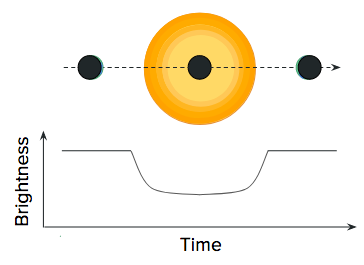
\includegraphics[width=0.3\linewidth]{Introduction/Figures/transit.png}
%     \caption{[TODO: use DejaVu Sans font for labels], [TODO: change planet color to black, because it should not be visible]}
%     \label{fig:transit}
% \end{figure}

\subsubsection{Transit timing variations}
\red{[TODO]}

\subsubsection{Radial velocity}
\red{[}This is arguably the most intuitive method\red{]}, as it aims to directly image a planet and resolve it from its host star. Although the idea is simple, in practice this method is challenged by the fact that the observed light from distant planetary systems is greatly dominated by the light emitted by the host star.
\subsubsection{Direct imaging}
By observing the light of a star at different wavelengths, its radial velocity can be inferred from shifts in the resulting spectrum. A change in radial velocity over time can be explained by the mutual interaction between an orbiting body and the star, causing the star to to move back and forth slightly in our line of sight. This method can also constrain the masses of the objects within the system.
\subsubsection{Microlensing}
A microlensing event occurs when a compact body such as a star acts as a lens and magnifies a more distant object in the background. This is due to the fact that the path of a ray of light is bent when it passes a massive body. In case a foreground star passes a background star in our line of sight, this effect should be visible for some duration as a peak in their combined brightness. Based on the signature of this change in brightness, one could infer whether a planet is likely to orbit the foreground star.

\subsection{Exoplanet-hunting missions}
Since the discovery of the first exoplanets, the rate at which exoplanets are detected has taken an exponential boost. Where at first it was the radial velocity method, it is now the transit method that holds most discoveries. At the time of writing, about one exoplanet is discovered every day over the past ten years on average by using the transit method. For all other methods combined, on average about one exoplanet is discovered every six days. The major turning point was when the search for transiting exoplanets was taken into space, and stars were monitored by the hundred thousands.

\subsubsection{Ground-based surveys}
\red{[TODO]}
\subsubsection{CoRoT}
\red{[TODO]}
\subsubsection{Kepler and K2}
With over 2500 exoplanet discoveries, Kepler and its continued mission ``K2'' are responsible for the detection of more than half of the known exoplanets. The Kepler space telescope has observed half a million stars in a small section of the sky. For most targets the cadence, or observation interval, was 30 minutes. A small fraction was observed with a cadence of one minute. Kepler operated for nearly ten years. Since its retirement in 2019, Kepler data is still a source for exoplanet discovery, as hidden and previously overlooked transit signals may yet to be detected \citep{hedges2019four}.

\subsubsection{TESS}
Launched in 2018, the Transiting Exoplanet Survey Satellite (TESS) has taken over the work of Kepler. As opposed to Kepler, TESS observes the full sky during its mission in the search for transiting exoplanets. It observes more brighter and closer targets than Kepler. TESS observations are of 2-minute cadence, though some targets are observed with a cadence of 20 seconds. Every 27.4 days, or sector, TESS changes its field of view. About halfway through each sector TESS links data down to Earth, during which no observations are made. At the time of writing, 125 exoplanet discoveries have resulted from TESS observations. With already over 200.000 stars observed, TESS is expected to discover thousands more.

\subsubsection{PLATO}
The PLAnetary Transits and Oscillations of stars (PLATO) mission will increase the numbers of several aspects. Planned for launch in 2026, this space-based telescope consisting of 34 \red{[TODO: fix, is less]} individual cameras will monitor up to a million stars. Its mission is to discover new transiting exoplanets and study their properties in greater depth. It will also perform asteroseismology to determine stellar parameters such as their mass. In combination with radial velocity measurements from the ground, this will allow for better characterization of the unknown worlds.